%% (Master) Thesis template
% Template version used: v1.4
%
% Largely adapted from Adrian Nievergelt's template for the ADPS
% (lecture notes) project.


%% We use the memoir class because it offers a many easy to use features.
\documentclass[11pt,a4paper,titlepage]{memoir}

%% Packages
%% ========

%% LaTeX Font encoding -- DO NOT CHANGE
\usepackage[OT1]{fontenc}

%% Babel provides support for languages.  'english' uses British
%% English hyphenation and text snippets like "Figure" and
%% "Theorem". Use the option 'ngerman' if your document is in German.
%% Use 'american' for American English.  Note that if you change this,
%% the next LaTeX run may show spurious errors.  Simply run it again.
%% If they persist, remove the .aux file and try again.
\usepackage[english]{babel}

%% Input encoding 'utf8'. In some cases you might need 'utf8x' for
%% extra symbols. Not all editors, especially on Windows, are UTF-8
%% capable, so you may want to use 'latin1' instead.
\usepackage[utf8]{inputenc}

%% This changes default fonts for both text and math mode to use Herman Zapfs
%% excellent Palatino font.  Do not change this.
\usepackage[sc]{mathpazo}

%% The AMS-LaTeX extensions for mathematical typesetting.  Do not
%% remove.
\usepackage{amsmath,amssymb,amsfonts,mathrsfs}

%% NTheorem is a reimplementation of the AMS Theorem package. This
%% will allow us to typeset theorems like examples, proofs and
%% similar.  Do not remove.
%% NOTE: Must be loaded AFTER amsmath, or the \qed placement will
%% break
\usepackage[amsmath,thmmarks]{ntheorem}

%% LaTeX' own graphics handling
\usepackage{graphicx}

%% We unfortunately need this for the Rules chapter.  Remove it
%% afterwards; or at least NEVER use its underlining features.
\usepackage{soul}

%% This allows you to add .pdf files. It is used to add the
%% declaration of originality.
\usepackage{pdfpages}

%% Some more packages that you may want to use.  Have a look at the
%% file, and consult the package docs for each.
%% See the TeXed file for more explanations

%% [OPT] Multi-rowed cells in tabulars
%\usepackage{multirow}

%% [REC] Intelligent cross reference package. This allows for nice
%% combined references that include the reference and a hint to where
%% to look for it.
\usepackage{varioref}

%% [OPT] Easily changeable quotes with \enquote{Text}
%\usepackage[german=swiss]{csquotes}

%% [REC] Format dates and time depending on locale
\usepackage{datetime}

%% [OPT] Provides a \cancel{} command to stroke through mathematics.
%\usepackage{cancel}

%% [NEED] This allows for additional typesetting tools in mathmode.
%% See its excellent documentation.
\usepackage{mathtools}

%% [ADV] Conditional commands
%\usepackage{ifthen}

%% [OPT] Manual large braces or other delimiters.
%\usepackage{bigdelim, bigstrut}

%% [REC] Alternate vector arrows. Use the command \vv{} to get scaled
%% vector arrows.
\usepackage[h]{esvect}

%% [NEED] Some extensions to tabulars and array environments.
\usepackage{array}

%% [OPT] Postscript support via pstricks graphics package. Very
%% diverse applications.
%\usepackage{pstricks,pst-all}

%% [?] This seems to allow us to define some additional counters.
%\usepackage{etex}

%% [ADV] XY-Pic to typeset some matrix-style graphics
%\usepackage[all]{xy}

%% [OPT] This is needed to generate an index at the end of the
%% document.
%\usepackage{makeidx}

%% [OPT] Fancy package for source code listings.  The template text
%% needs it for some LaTeX snippets; remove/adapt the \lstset when you
%% remove the template content.
\usepackage{listings}
\lstset{language=TeX,basicstyle={\normalfont\ttfamily}}

%% [REC] Fancy character protrusion.  Must be loaded after all fonts.
\usepackage[activate]{pdfcprot}

%% [REC] Nicer tables.  Read the excellent documentation.
\usepackage{booktabs}


%% Our layout configuration.  DO NOT CHANGE.
%% Memoir layout setup

%% NOTE: You are strongly advised not to change any of them unless you
%% know what you are doing.  These settings strongly interact in the
%% final look of the document.

% Dependencies
\usepackage{ETHlogo}

% Turn extra space before chapter headings off.
\setlength{\beforechapskip}{0pt}

\nonzeroparskip
\parindent=0pt
\defaultlists

% Chapter style redefinition
\makeatletter

\if@twoside
  \pagestyle{Ruled}
  \copypagestyle{chapter}{Ruled}
\else
  \pagestyle{ruled}
  \copypagestyle{chapter}{ruled}
\fi
\makeoddhead{chapter}{}{}{}
\makeevenhead{chapter}{}{}{}
\makeheadrule{chapter}{\textwidth}{0pt}
\copypagestyle{abstract}{empty}

\makechapterstyle{bianchimod}{%
  \chapterstyle{default}
  \renewcommand*{\chapnamefont}{\normalfont\Large\sffamily}
  \renewcommand*{\chapnumfont}{\normalfont\Large\sffamily}
  \renewcommand*{\printchaptername}{%
    \chapnamefont\centering\@chapapp}
  \renewcommand*{\printchapternum}{\chapnumfont {\thechapter}}
  \renewcommand*{\chaptitlefont}{\normalfont\huge\sffamily}
  \renewcommand*{\printchaptertitle}[1]{%
    \hrule\vskip\onelineskip \centering \chaptitlefont\textbf{\vphantom{gyM}##1}\par}
  \renewcommand*{\afterchaptertitle}{\vskip\onelineskip \hrule\vskip
    \afterchapskip}
  \renewcommand*{\printchapternonum}{%
    \vphantom{\chapnumfont {9}}\afterchapternum}}

% Use the newly defined style
\chapterstyle{bianchimod}

\setsecheadstyle{\Large\bfseries\sffamily}
\setsubsecheadstyle{\large\bfseries\sffamily}
\setsubsubsecheadstyle{\bfseries\sffamily}
\setparaheadstyle{\normalsize\bfseries\sffamily}
\setsubparaheadstyle{\normalsize\itshape\sffamily}
\setsubparaindent{0pt}

% Set captions to a more separated style for clearness
\captionnamefont{\sffamily\bfseries\footnotesize}
\captiontitlefont{\sffamily\footnotesize}
\setlength{\intextsep}{16pt}
\setlength{\belowcaptionskip}{1pt}

% Set section and TOC numbering depth to subsection
\setsecnumdepth{subsection}
\settocdepth{subsection}

%% Titlepage adjustments
\pretitle{\vspace{0pt plus 0.7fill}\begin{center}\HUGE\sffamily\bfseries}
\posttitle{\end{center}\par}
\preauthor{\par\begin{center}\let\and\\\Large\sffamily}
\postauthor{\end{center}}
\predate{\par\begin{center}\Large\sffamily}
\postdate{\end{center}}

\def\@advisors{}
\newcommand{\advisors}[1]{\def\@advisors{#1}}
\def\@department{}
\newcommand{\department}[1]{\def\@department{#1}}
\def\@thesistype{}
\newcommand{\thesistype}[1]{\def\@thesistype{#1}}

\renewcommand{\maketitlehooka}{\noindent\ETHlogo[2in]}

\renewcommand{\maketitlehookb}{\vspace{1in}%
  \par\begin{center}\Large\sffamily\@thesistype\end{center}}

\renewcommand{\maketitlehookd}{%
  \vfill\par
  \begin{flushright}
    \sffamily
    \@advisors\par
    \@department, ETH Z\"urich
  \end{flushright}
}

\checkandfixthelayout

\setlength{\droptitle}{-48pt}

\makeatother

% This defines how theorems should look. Best leave as is.
\theoremstyle{plain}
\setlength\theorempostskipamount{0pt}

%%% Local Variables:
%%% mode: latex
%%% TeX-master: "thesis"
%%% End:


%% Theorem environments.  You will have to adapt this for a German
%% thesis.
%% Theorem-like environments

%% This can be changed according to language. You can comment out the ones you
%% don't need.

\numberwithin{equation}{chapter}

%% German theorems
%\newtheorem{satz}{Satz}[chapter]
%\newtheorem{beispiel}[satz]{Beispiel}
%\newtheorem{bemerkung}[satz]{Bemerkung}
%\newtheorem{korrolar}[satz]{Korrolar}
%\newtheorem{definition}[satz]{Definition}
%\newtheorem{lemma}[satz]{Lemma}
%\newtheorem{proposition}[satz]{Proposition}

%% English variants
\newtheorem{theorem}{Theorem}[chapter]
\newtheorem{example}[theorem]{Example}
\newtheorem{remark}[theorem]{Remark}
\newtheorem{corollary}[theorem]{Corollary}
\newtheorem{definition}[theorem]{Definition}
\newtheorem{lemma}[theorem]{Lemma}
\newtheorem{proposition}[theorem]{Proposition}

%% Proof environment with a small square as a "qed" symbol
\theoremstyle{nonumberplain}
\theorembodyfont{\normalfont}
\theoremsymbol{\ensuremath{\square}}
\newtheorem{proof}{Proof}
%\newtheorem{beweis}{Beweis}


%% Helpful macros.
%% Custom commands
%% ===============

%% Special characters for number sets, e.g.\ real or complex numbers.
\newcommand{\C}{\mathbb{C}}
\newcommand{\K}{\mathbb{K}}
\newcommand{\N}{\mathbb{N}}
\newcommand{\Q}{\mathbb{Q}}
\newcommand{\R}{\mathbb{R}}
\newcommand{\Z}{\mathbb{Z}}
\newcommand{\X}{\mathbb{X}}

%% Fixed/scaling delimiter examples (see mathtools documentation)
\DeclarePairedDelimiter\abs{\lvert}{\rvert}
\DeclarePairedDelimiter\norm{\lVert}{\rVert}

%% Use the alternative epsilon per default and define the old one as \oldepsilon
\let\oldepsilon\epsilon
\renewcommand{\epsilon}{\ensuremath\varepsilon}

%% Also set the alternate phi as default.
\let\oldphi\phi
\renewcommand{\phi}{\ensuremath{\varphi}}

%% Create argmax and argmin operators.
%% Thin space, limits underneath in displays.
\DeclareMathOperator*{\argmin}{arg\,min}
%% Thin space, limits underneath in displays.
\DeclareMathOperator*{\argmax}{arg\,max}


%% Make document internal hyperlinks wherever possible. (TOC, references)
%% This MUST be loaded after varioref, which is loaded in 'extrapackages'
%% above.  We just load it last to be safe.
\usepackage[linkcolor=black,colorlinks=true,citecolor=black,filecolor=black]{hyperref}


%% Document information
%% ====================

\title{Title of Thesis}
\author{S. Tudent}
\thesistype{Master Thesis}
\advisors{Advisors: Prof.\ Dr.\ A. D. Visor, Dr.\ P. Ostdoc}
\department{Department of Computer Science}
\date{January 19, 2038}

\begin{document}

\frontmatter

%% Title page is autogenerated from document information above.  DO
%% NOT CHANGE.
\begin{titlingpage}
  \calccentering{\unitlength}
  \begin{adjustwidth*}{\unitlength-24pt}{-\unitlength-24pt}
    \maketitle
  \end{adjustwidth*}
\end{titlingpage}

%% The abstract of your thesis.  Edit the file as needed.
\begin{abstract}
  ~150 words
  % 1 Top-m arm identification comprehensible for any scientist
  Top-$m$ arm revolves around identifying the set of $m$ best options with rewards following unknown probability distributions through the draw of samples.
  % 2 Top-m arm identification comprehensible for scientist from the field
  In particular, for a fixed budget of samples, one seeks to increase confidence in the estimate. Conversely, for a fixed confidence, one seeks to require the least amount of samples possible. Hence the optimization revolves around a fast convergence rate of the confidence for increasing samples.
  %1 The problem addressed by this paper
  Our work seeks to characterize this optimality concept more explicitly and intuitively as well as provide an algorithm which is promising to converge to said optimality.
  % 1 Summary of main result
  Our characterization, relying on a definition of evidence, proves that the optimal allocation collects equal evidence to distinguish every pair of optimal and suboptimal arms.
  % 2 How the main result changes previous knowledge
  This characterization allows for a better intuitive understanding of the top-$m$ mechanism and should make it more convenient to prove convergence of algorithms. Being very simplistic to understand and implement, our algorithm comes with confidence estimates and allows for leveraging prior knowledge.
  %!1 Result in general context
  %2 Broader perspective, understandable by any scientist
  We hope that this work lays the foundation for top-$m$ convergence proofs, in particular for our suggested algorithm.
\end{abstract}


%% TOC with the proper setup, do not change.
\cleartorecto
\tableofcontents
\mainmatter

%% Your real content!
% Some commands used in this file
\newcommand{\package}{\emph}

\chapter{Introduction}

% \begin{itemize}
%   \item Algorithm and characterization for top-m arm identification as a generalization of Russo's top-1 work.
%   \item What is the relationship between the optimal allocation and the algorithm?
%   \item Talk about optimal (fixed) vs adaptive.
%   $\rightarrow$ Mention the the outlook of proving convergence based on results
%   we've established.
%   \item Algorithm details/constraints:
%   \begin{itemize}
%     \item What are constraints on prior and posterior distributions?
%     \item Are we in a frequentist or Bayesian setting?
%     \item What is particular about the algorithm being Bayesian?
%   \end{itemize}
%   \item How do both statements translate to real world applications?
%   \item Explain the flow of the document.
% \end{itemize}


Much of Machine Learning revolves around how to learn from observations. On the one hand, technological advances allow for an extensive gathering of data in a pluratily of domains. On the other hand, many domains are still, and likely to remain, areas of expensive data acquisition. Due to immense complexity, human behaviour as well as many physical processes can only be simulated at very high costs or not at all. As a consequence, data is gathered by experiments that can be long-lasting, strictly constrained in quantity and precious. In light of that, we focus on the following aspect of Machine Learning: how to acquire observations.

In order to capture the complexity of real-world processes, we model outcomes of decisions according to probability distributions. More precisely, we make use of the well-established multi-armed bandits model for that exact purpose. As we've mentioned, we seek to describe a manner of acquiring, or sampling, observations. Naturally, one must ask the question: 'With what exact goal?'

We assume the goal of the data generation and acquisition to be the identification of the $m$ best options. Within the realm of this goal, we tackle problems:
\begin{itemize}
  \item What is, in theory, the best possible acquisition strategy?
  \item What can be algorithm that can, under some constraints, mimics this best possible acquisition strategy?
\end{itemize}
In particular, we seek to address these challenges by generalizing work from Russo \cite{DBLP:journals/corr/Russo16} on best arm identification.

We assume a frequentist setting. This implies that the options follow fixed distributions, which are unknown to us. Yet, we can sample from those distributions. This can be thought of as being confronted with a noise-free signal that is then polluted with noise from a sensor. In this spirit, we seek to identify the true best options with as few samples as possible and be as confident of our recommendation as possible.

Our first contribution is the characterization of the optimal acquisition strategy, also referred to as measurement plan or allocation. What makes the optimal allocation optimal is the rate of increase in confidence in the true best options per sample. This optimal strategy is based on a thought experiment of knowing the underlying truth and acquiring samples validating the knowledge as well as possible. As a consequence, it serves as a bound for practical algorithms outside of thought experiments. Intuitively, the guiding theme of the characterization is that the allocation seeks to gather equal \emph{evidence} on every option.

Our second contribution is the definition of a concrete and simple adaptive algorithm. As compared to the optimal allocation, the algorithm changes its measurement plan after every sample, based on the observations it has made. The algorithm being Bayesian, it comes with the upside of confidence estimation and allows for leveraging and expressing domain knowledge through the use of priors. We analyze properties of the algorithm and highlight insights that we deem very useful for proving asymptotic convergence of this algorithm's allocation to the optimal allocation.

In those undertakings we make very few assumptions on the underlying conditions. Concretely, we expect the options to follow distributions from the
one-dimensional canonical exponential family. This includes common distributions such as the Bernoulli, binomial with known number of trials, Poisson, exponential, Pareto with known minimal value, chi-squared or the normal distribution with known variance.

\Cref{chapter:background} introduces the general problem context as well as Russo's work we attempt to generalize to top-$m$ selection. We characterize the optimal allocation in \Cref{chapter:optimal}. Our proposed algorithm, Top-2$m$ XOR Thompson sampling, is presented and analyzed in \Cref{chapter:algorithm} before concluding our work in \Cref{chapter:conclusion}.

\chapter{Writing scientific texts in English}

This chapter was originally a separate document written by Reto
Spöhel.  It is reprinted here so that the template can serve as a
quick guide to thesis writing, and to provide some more example
material to give you a feeling for good typesetting.

% We're going to need an extra theorem-like environment for this
% chapter
\theoremstyle{plain}
\theoremsymbol{}
\newtheorem{Rule}[theorem]{Rule}

\section{Basic writing rules}

The following rules need little further explanation; they are best
understood by looking at the example in the booklet by Knuth et al.,
§2--§3.

\begin{Rule}
  Write texts, not chains of formulas.
\end{Rule}

More specifically, write full sentences that are logically
interconnected by phrases like `Therefore', `However', `On the other
hand', etc.\ where appropriate.

\begin{Rule}
  Displayed formulas should be embedded in your text and punctuated
  with it.
\end{Rule}

In other words, your writing should not be divided into `text parts'
and `formula parts'; instead the formulas should be tied together by
your prose such that there is a natural flow to your writing.

\section{Being nice to the reader}

Try to write your text in such a way that a reader enjoys reading
it. That's of course a lofty goal, but nevertheless one you should
aspire to!

\begin{Rule}
  Be nice to the reader.
\end{Rule}

Give some intuition or easy example for definitions and theorems which
might be hard to digest. Remind the reader of notations you introduced
many pages ago -- chances are he has forgotten them. Illustrate your
writing with diagrams and pictures where this helps the reader. Etc.

\begin{Rule}
  Organize your writing.
\end{Rule}

Think carefully about how you subdivide your thesis into chapters,
sections, and possibly subsections.  Give overviews at the beginning
of your thesis and of each chapter, so the reader knows what to
expect. In proofs, outline the main ideas before going into technical
details. Give the reader the opportunity to `catch up with you' by
summing up your findings periodically.

\emph{Useful phrases:} `So far we have shown that \ldots', `It remains
to show that \ldots', `Recall that we want to prove inequality (7), as
this will allow us to deduce that \ldots', `Thus we can conclude that
\ldots. Next, we would like to find out whether \ldots', etc.

\begin{Rule}
  Don't say the same thing twice without telling the reader that you
  are saying it twice.
\end{Rule}

Repetition of key ideas is important and helpful. However, if you
present the same idea, definition or observation twice (in the same or
different words) without telling the reader, he will be looking for
something new where there is nothing new.

\emph{Useful phrases:} `Recall that [we have seen in Chapter 5 that]
\ldots', `As argued before / in the proof of Lemma 3, \ldots', `As
mentioned in the introduction, \ldots', `In other words, \ldots', etc.

\begin{Rule}
  Don't make statements that you will justify later without telling
  the reader that you will justify them later.
\end{Rule}

This rule also applies when the justification is coming right in the
next sentence!  The reasoning should be clear: if you violate it, the
reader will lose valuable time trying to figure out on his own what
you were going to explain to him anyway.

\emph{Useful phrases:} `Next we argue that \ldots', `As we shall see,
\ldots', `We will see in the next section that \ldots, etc.


\section{A few important grammar rules}

\begin{Rule}
  \label{rule:no-comma-before-that}
  There is (almost) \emph{never} a comma before `that'.
\end{Rule}

It's really that simple. Examples:
\begin{quote}
  We assume that \ldots\\
  \emph{Wir nehmen an, dass \ldots}

  It follows that \ldots\\
  \emph{Daraus folgt, dass \ldots}

  `thrice' is a word that is seldom used.\\
  \emph{`thrice' ist ein Wort, das selten verwendet wird.}
\end{quote}
Exceptions to this rule are rare and usually pretty obvious. For
example, you may end up with a comma before `that' because `i.e.\' is
spelled out as `that is':
\begin{quote}
  For \(p(n)=\log n/n\) we have \ldots{} However, if we choose \(p\) a
  little bit higher, that is \(p(n)=(1+\varepsilon)\log n/n\) for some
  \(\varepsilon>0\), we obtain that\ldots
\end{quote}
Or you may get a comma before `that' because there is some additional
information inserted in the middle of your sentence:
\begin{quote}
  Thus we found a number, namely \(n_0\), that satisfies equation (13).
\end{quote}
If the additional information is left out, the sentence has no comma:
\begin{quote}
  Thus we found a number that satisfies equation (13).
\end{quote}
(For `that' as a relative pronoun, see also
Rules~\ref{rule:non-defining-has-comma}
and~\ref{rule:defining-without-comma} below.)

\begin{Rule}
  There is usually no comma before `if'.
\end{Rule}

Example:
\begin{quote}
  A graph is not \(3\)-colorable if it contains a \(4\)-clique.\\
  \emph{Ein Graph ist nicht \(3\)-färbbar, wenn er eine \(4\)-Clique
    enthält.}
\end{quote}
However, if the `if' clause comes first, it is usually separated from
the main clause by a comma:
\begin{quote}
  If a graph contains a \(4\)-clique, it is not \(3\)-colorable .\\
  \emph{Wenn ein Graph eine \(4\)-Clique enthält, ist er nicht
    \(3\)-färbbar.}
\end{quote}

There are more exceptions to these rules than to
Rule~\ref{rule:no-comma-before-that}, which is why we are not
discussing them here. Just keep in mind: don't put a comma before `if'
without good reason.

\begin{Rule}
  \label{rule:non-defining-has-comma}
  Non-defining relative clauses have commas.
\end{Rule}
\begin{Rule}
  \label{rule:defining-without-comma}
  Defining relative clauses have no commas.
\end{Rule}

In English, it is very important to distinguish between two types of
relative clauses: defining and non-defining ones. This is a
distinction you absolutely need to understand to write scientific
texts, because mistakes in this area actually distort the meaning of
your text!

It's probably easier to explain first what a \emph{non-defining}
relative clause is. A non-defining relative clauses simply gives
additional information \emph{that could also be left out} (or given in
a separate sentence). For example, the sentence
\begin{quote}
  The \textsc{WeirdSort} algorithm, which was found by the famous
  mathematician John Doe, is theoretically best possible but difficult
  to implement in practice.
\end{quote}
would be fully understandable if the relative clause were left out
completely. It could also be rephrased as two separate sentences:
\begin{quote}
  The \textsc{WeirdSort} algorithm is theoretically best possible but
  difficult to implement in practice. [By the way,] \textsc{WeirdSort}
  was found by the famous mathematician John Doe.
\end{quote}
This is what a non-defining relative clause is. \emph{Non-defining
  relative clauses are always written with commas.} As a corollary we
obtain that you cannot use `that' in non-defining relative clauses
(see Rule~\ref{rule:no-comma-before-that}!). It would be wrong to
write
\begin{quote}
  \st{The \textsc{WeirdSort} algorithm, that was found by the famous
    mathematician John Doe, is theoretically best possible but
    difficult to implement in practice.}
\end{quote}
A special case that warrants its own example is when `which' is
referring to the entire preceding sentence:
\begin{quote}
  Thus inequality (7) is true, which implies that the Riemann
  hypothesis holds.
\end{quote}
As before, this is a non-defining relative sentence (it could be left
out) and therefore needs a comma.

So let's discuss \emph{defining} relative clauses next. A defining
relative clause tells the reader \emph{which specific item the main
  clause is talking about}. Leaving it out either changes the meaning
of the sentence or renders it incomprehensible altogether.  Consider
the following example:

\begin{quote}
  The \textsc{WeirdSort} algorithm is difficult to implement in
  practice. In contrast, the algorithm that we suggest is very simple.
\end{quote}

Here the relative clause `that we suggest' cannot be left out -- the
remaining sentence would make no sense since the reader would not know
which algorithm it is talking about. This is what a defining relative
clause is. \textit{Defining relative clauses are never written with
  commas.} Usually, you can use both `that' and `which' in defining
relative clauses, although in many cases `that' sounds better.

As a final example, consider the following sentence:
\begin{quote}
  For the elements in \(\mathcal{B}\) which satisfy property (A), we
  know that equation (37) holds.
\end{quote}
This sentence does not make a statement about all elements in
\(\mathcal{B}\), only about those satisfying property (A). The relative
clause is \emph{defining}. (Thus we could also use `that' in place of
`which'.)

In contrast, if we add a comma the sentence reads
\begin{quote}
  For the elements in \(\mathcal{B}\), which satisfy property (A), we
  know that equation (37) holds.
\end{quote}

Now the relative clause is \emph{non-defining} -- it just mentions in
passing that all elements in \(\mathcal{B}\) satisfy property (A). The
main clause states that equation (37) holds for \emph{all} elements in
\(\mathcal{B}\). See the difference?


\section[Things you (usually) don't say in English]%
{Things you (usually) don't say in English -- and what to say
  instead}
\label{sec:list}

Table~\ref{tab:things-you-dont-say} lists some common mistakes and
alternatives.  The entries should not be taken as gospel -- they don't
necessarily mean that a given word or formulation is wrong under all
circumstances (obviously, this depends a lot on the context). However,
in nine out of ten instances the suggested alternative is the better
word to use.

\begin{table}
  \centering
  \caption{Things you (usually) don't say}
  \label{tab:things-you-dont-say}
  \begin{tabular}{lll}
    \toprule
    \st{It holds (that) \dots} & We have \dots & \emph{Es gilt \dots}\\
    \multicolumn{3}{l}{\quad\footnotesize(`Equation (5) holds.' is fine, though.)}\\
    \st{$x$ fulfills property $\mathcal{P}$.}& \(x\) satisfies property \(\mathcal{P}\). & \emph{\(x\) erfüllt Eigenschaft \(\mathcal{P}\).} \\
    \st{in average} & on average & \emph{im Durchschnitt}\\
    \st{estimation} & estimate   & \emph{Abschätzung}\\
    \st{composed number} & composite number & \emph{zusammengesetzte Zahl}\\
    \st{with the help of} & using & \emph{mit Hilfe von}\\
    \st{surely} & clearly & \emph{sicher, bestimmt}\\
    \st{monotonously increasing} & monotonically incr. & \emph{monoton steigend}\\
    \multicolumn{3}{l}{\quad\footnotesize(Actually, in most cases `increasing' is just fine.)}\\
    \bottomrule
  \end{tabular}
\end{table}

%%% Local Variables:
%%% mode: latex
%%% TeX-master: "thesis"
%%% End:

\chapter{Typography}


\section{Punctuation}

\begin{Rule}
  Use opening (`) and closing (') quotation marks correctly.
\end{Rule}

In \LaTeX, the closing quotation mark is typed like a normal
apostrophe, while the opening quotation mark is typed using the French
\emph{accent grave} on your keyboard (the \emph{accent grave} is the
one going down, as in \emph{frère}).

Note that any punctuation that \emph{semantically} follows quoted
speech goes inside the quotes in American English, but outside in
Britain.  Also, Americans use double quotes first.  Oppose
\begin{quote}
  ``Using `lasers,' we punch a hole in \ldots\ the Ozone Layer,''
  Dr.\ Evil said.
\end{quote}
to
\begin{quote}
  `Using ``lasers'', we punch a hole in \ldots\ the Ozone Layer',
  Dr.\ Evil said.
\end{quote}

\begin{Rule}
  Use hyphens (-), en-dashes (--) and em-dashes (---) correctly.
\end{Rule}

A hyphen is only used in words like `well-known', `$3$-colorable'
etc., or to separate words that continue in the next line (which is
known as hyphenation).  It is entered as a single ASCII hyphen
character (\texttt{-}).

To denote ranges of numbers, chapters, etc., use an en-dash (entered
as two ASCII hyphens \texttt{--}) with no spaces on either side.  For
example, using Equations (1)--(3), we see\ldots

As the equivalent of the German \emph{Gedankenstrich}, use an en-dash
with spaces on both sides -- in the title of Section \ref{sec:list},
it would be wrong to use a hyphen instead of the dash. (Some English
authors use the even longer emdash (---) instead, which is typed as
three subsequent hyphens in \LaTeX. This emdash is used without spaces
around it---like so.)


\section{Spacing}

\begin{Rule}
  \label{rule:no-manual-spacing}
  Do not add spacing manually.
\end{Rule}

You should never use the commands \lstinline-\\- (except within
tabulars and arrays), \lstinline[showspaces=true]-\ - (except to
prevent a sentence-ending space after Dr.\ and such),
\lstinline-\vspace-, \lstinline-\hspace-, etc.  The choices programmed
into \LaTeX{} and this style should cover almost all cases.  Doing it
manually quickly leads to inconsistent spacing, which looks terrible.
Note that this list of commands is by no means conclusive.

\begin{Rule}
  Judiciously insert spacing in maths where it helps.
\end{Rule}

This directly contradicts Rule~\ref{rule:no-manual-spacing}, but in
some cases \TeX{} fails to correctly decide how much spacing is
required.  For example, consider
\begin{displaymath}
  f(a,b) = f(a+b, a-b).
\end{displaymath}
In such cases, inserting a thin math space \lstinline-\,- greatly
increases readability:
\begin{displaymath}
  f(a,b) = f(a+b,\, a-b).
\end{displaymath}

Along similar lines, there are variations of some symbols with
different spacing.  For example, Lagrange's Theorem states that
\(\abs{G}=[G:H]\abs{H}\), but the proof uses a bijection \(f\colon
aH\to bH\).  (Note how the first colon is symmetrically spaced, but
the second is not.)

\begin{Rule}
  Learn when to use \lstinline[showspaces=true]-\ - and
  \lstinline-\@-.
\end{Rule}

Unless you use `french spacing', the space at the end of a sentence is
slightly larger than the normal interword space.

The rule used by \TeX{} is that any space following a period,
exclamation mark or question mark is sentence-ending, except for
periods preceded by an upper-case letter.  Inserting \lstinline-\-
before a space turns it into an interword space, and inserting
\lstinline-\@- before a period makes it sentence-ending.  This means
you should write
\begin{lstlisting}
Prof.\ Dr.\ A. Steger is a member of CADMO\@.
If you want to write a thesis with her, you
should use this template.
\end{lstlisting}
which turns into
\begin{quote}
  Prof.\ Dr.\ A. Steger is a member of CADMO\@.  If you want to write
  a thesis with her, you should use this template.
\end{quote}
The effect becomes more dramatic in lines that are stretched slightly
during justification:
\begin{quote}
  \parbox{\linewidth}{\hbox to \linewidth{%
      Prof.\ Dr.\ A. Steger is a member of CADMO\@.  If you}}
\end{quote}

\begin{Rule}
  Place a non-breaking space (\lstinline-~-) right before references.
\end{Rule}

This is actually a slight simplification of the real rule, which
should invoke common sense.  Place non-breaking spaces where a line
break would look `funny' because it occurs right in the middle of a
construction, especially between a reference type (Chapter) and its
number.


\section{Choice of `fonts'}

Professional typography distinguishes many font attributes, such as
family, size, shape, and weight.  The choice for sectional divisions
and layout elements has been made, but you will still occasionally
want to switch to something else to get the reader's attention.  The
most important rule is very simple.

\begin{Rule}
  When emphasising a short bit of text, use \lstinline-\emph-.
\end{Rule}

In particular, \emph{never} use bold text (\lstinline-\textbf-).
Italics (or Roman type if used within italics) avoids distracting the
eye with the huge blobs of ink in the middle of the text that bold
text so quickly introduces.

Occasionally you will need more notation, for example, a consistent
typeface used to identify algorithms.

\begin{Rule}
  Vary one attribute at a time.
\end{Rule}

For example, for \textsc{WeirdSort} we only changed the shape to small
caps.  Changing two attributes, say, to bold small caps would be
excessive (\LaTeX{} does not even have this particular variation).
The same holds for mathematical notation: the reader can easily
distinguish \(g_n\), \(G(x)\), \(\mathcal{G}\) and \(\mathsf{G}\).

\begin{Rule}
  Never underline or uppercase.
\end{Rule}

No exceptions to this one, unless you are writing your thesis on a
typewriter.  Manually.  Uphill both ways.  In a blizzard.


\section{Displayed equations}

\begin{Rule}
  Insert paragraph breaks \emph{after} displays only where they
  belong.  Never insert paragraph breaks \emph{before} displays.
\end{Rule}

\LaTeX{} translates sequences of more than one linebreak (i.e.\, what
looks like an empty line in the source code) into a paragraph break in
almost all contexts.  This also happens before and after displays,
where extra spacing is inserted to give a visual indication of the
structure.  Adding a blank line in these places may look nice in the
sources, but compare the resulting display

\begin{displaymath}
  a = b
\end{displaymath}

to the following:
\begin{displaymath}
  a = b
\end{displaymath}
The first display is surrounded by blank lines, but the second is not.
It is bad style to start a paragraph with a display (you should always
tell the reader what the display means first), so the rule follows.

\begin{Rule}
  Never use \lstinline-eqnarray-.
\end{Rule}

It is at the root of most ill-spaced multiline displays.  The
\package{amsmath} package provides better alternatives, such as the
\lstinline-align- family
\begin{align*}
  f(x) &= \sin x, \\
  g(x) &= \cos x,
\end{align*}
and \lstinline-multline- which copes with excessively long equations:
\begin{multline*}
  \def\P{\mathrm P}
  \P\bigl[X_{t_0} \in (z_0, z_0+dz_0],\ldots, X_{t_n}\in(z_n,z_n+dz_n]\bigr]
  \\= \nu(dz_0) K_{t_1}(z_0,dz_1) K_{t_2-t_1}(z_1,dz_2)\cdots
  K_{t_n-t_{n-1}}(z_{n-1},dz_n).
\end{multline*}


\section{Floats}

By default this style provides floating environments for tables and
figures.  The general structure should be as follows:
\begin{lstlisting}
\begin{figure}
  \centering
  % content goes here
  \caption{A short caption}
  \label{some-short-label}
\end{figure}
\end{lstlisting}
Note that the label must follow the caption, otherwise the label will
refer to the surrounding section instead.  Also note that figures
should be captioned at the bottom, and tables at the top.

The whole point of floats is that they, well, \emph{float} to a place
where they fit without interrupting the text body.  This is a frequent
source of confusion and changes; please leave it as is.

\begin{Rule}
  Do not restrict float movement to only `here'
  \textnormal{(\lstinline-h-)}.
\end{Rule}

If you are still tempted, you should avoid the float altogether and
just show the figure or table inline, similar to a displayed equation.

%%% Local Variables:
%%% mode: latex
%%% TeX-master: "thesis"
%%% End:

\chapter{Background}

\section{Chernoff's 2-player game}
Tbd whether relevant.

\section{Bandits}
%What is the scenario/model?
The so-called stochastic multi-armed bandits is a general model to simulate decision-making in uncertain environments.
In particular, one assumes a set of options or arms to choose from, each choice leading to an outcome, also referred to as reward. In general, one assumes many sequential selections among the set of arms. It is typically assumed that the outcome of the selection of an individual arm follows a fixed but unknown probability distribution.

%What problems are typically tackled by this scenario?
Within the bandits model, the concern revolves around which arm to choose next. Allocation strategies tackling this question address either of two problems: explore-exploit or pure-explore.

The former concerns itself with maximizing the \emph{cummulative reward}. This means that one attempts to maximize the \emph{sum of the rewards obtained} through all arm selections. Naturally, starting off without any knowledge about the underlying distributions, this involves both exploration of arm qualities as well as exploitation of gathered knowledge.

The latter revolves around \emph{simple reward}. This problem consists of seeking to maximize the reward one obtains if one leverages the current knowledge for \emph{another} draw. This implies that the focus lies on \emph{identification} of high-quality candidates, where quality is usually assessed by high means. Hence it is part of the task to make estimated best and true best equal as well as obtaining a high \emph{confidence} on this statement.

%Why is model and its problems relevant?
The bandits model can be used for all processes involving sequential decision making. Yet, an important simplification is the assumption of the distributions being fixed over time. This assumption might be more or less representative of the true, to-be-modelled processes.

The explore-exploit problem is applied in Recommender Systems, ad campaigns, in the context of Reinforcement Learning and Robotics.

For real-world applications of the pure-exploration bandit please refer to \ref{ss:top-1_model}.

There exist many specialized versions of the Bandits model, such as contextual bandits or adversarial bandits.

\section{Thompson Sampling}
%How does it work?
%Why is it useful?
%What is it used for?

Thompson sampling is a sampling strategy often employed for choosing arms in the bandits scenario. By default, it particularly lends itself to the cummulative reward setting. The technique is based on having and updating prior distributions over all arms. In contrast to greedily selecting the arm that empirically maximizes the metric of desire, Thompson sampling suggests to randomly draw beliefs on arms from the prior distributions. Subsequently, it selects the arm which maximizes the metric of desire on the sampled belief.
With many repetitions, this leads to each arm being sampled proportionally to its likelihood of maximizing the metric of desire according to current belief.
Intuitively, this is very appealing for the cummulative reward scenario as it creates a natural balance between exploration and exploitation.

% Insert algorithm from overview paper?

\section{Notation}
%TODO: Talk about deq.

We assume $k$ arms to choose from and denote the set of possible arms as $[k]$. Subsets $S \subset [k]$ are assumed to be of size $m < k$.

A possible set of means for the arms is denoted as the $k$-dimensional vector $\theta$, where every mean can lie between 0 and 1. We also refer to such a $\theta$ as parameter.

Finding ourselves in a frequentist setting, we assume an underlying true mean of the arms refer to this as $\theta^*$. Moreover, this ground truth implies a true best arm $l^*$ and true top-$m$ arms $S^*$. When referring to an individual arm in the top-$m$ case, we proceed to use $j$ for arms in $S^*$, $i$ for arms not in $S^*$ and $l$ for arms of which this knowledge does not exist.

Given the constraint that the means lie between 0 and 1, there are infinitely many possible parameter vectors which make arm $l \in [k]$ the best one under $\theta$ or $S \subset [k]$ top-$m$ under $\theta$. Hence we group such $\theta$ in the following way:
\begin{align}
  \Theta &:= [0, 1]^k \\
  \Theta_{1, l} &:= \{\theta \in \Theta | l = \argmax_{l' \in [k]} \theta_{l'}\} \\
  \Theta_{m, S} &:= \{\theta \in \Theta | S = \text{top-}m(\theta)\} \\
    &= \{ \theta \in \Theta| \min_{j_1 \in S}\ \theta_{j_1} > \max_{j_2 \notin S}\ \theta_{j_2}\} \\
  \Theta_{m, l} &= \{\theta \in \Theta | l \in \text{ top-}m(\theta)\}
\end{align}
where top-$m$ returns the $m$ highest values, i.e. means, from its argument $\theta$.

After having made $n$ observations of rewards, bundled in $D_n$, $\Pi_n$ expresses a posterior distribution with density $\pi_n$ over elements of $\Theta$. E.g. for sets $\Theta_{m, S}$, we have:
\begin{align}
  \Pi_n(\Theta_{m, S}) &:= \int_{\theta \in \Theta_{m, S}} \pi_n(\theta) d\theta \\
    &= \Pr[S \text{ is top-}m | D_n]
\end{align}
Clearly, it holds that $\Pi_n(\Theta) = 1$. As a shorthand for the top-$m$ case, we will use:
\begin{align}
  \alpha_{n, l} &:= \Pi_n(\Theta_{m, l}) \\
  \alpha_{n, S} &:= \Pi_n(\Theta_{m, S})
\end{align}
We are mostly interested in strategies that allocate measurement effort over the arms in a randomized fashion, i.e. according to a probability distribution. We refer to such an allocation or distribution as $\psi$, defining the probability of each arm being sampled. Naturally, it holds that $\sum_{l \in [k]} \psi_l = 1$.

The $n$-th sampled arm is denoted as $l_n$. For adaptive strategies, the allocation can change after every sample. After $n$ sample we refer to the allocation s as $\psi_{n}$ and therefore after $n$ samples we have $\psi_{n, l} = \Pr[l_n = l]$ for arm $l$. We also define the allocation property of a set by the sum of its arms: $\psi_S = \sum_{l \in S} \psi_l$. In the case of adaptive strategies, we might as well be interested in average allocation up to a certain sample $n$. We write:
\begin{align}
  \bar{\psi}_{n, l} &:= \frac{\sum_{n' = 1}^{n} \psi_{n', l}}{n}
\end{align}
We use the notation $d(\theta_1||\theta_2)$ to represent the Kullback-Leibler divergence between $\theta_1$ and $\theta_2$.

\section{Best Arm Identification}
\subsection{Model}\label{ss:top-1_model}
%What is the problem?
%Why is it relevant?
%How is performance evaluated? What is 'confidence'?

Best Arm identification implies disregarding the sum of the rewards encountered while sampling. Rather, the goal is to efficiently gather information maximizing the confidence of the suggestion made \emph{after} the sampling phase. In other words, there is a purely explorative phase, also referred to as 'experiment' which is then typically followed by a purely exploitative phase, having committed to an option. For this reason, Best Arm Identification is also known as 'Experiment Design'.

Quite naturally, all other aspects being controlled for, requiring fewer samples is preferable. Hence one can formulate the goal in two ways: maximize confidence for a fix amount of samples or minimize amount of samples for a fixed confidence.

Confidence can mean and be evaluated in different ways. For Bayesian algorithms, it is possible to quantify the confidence the model has in the currently most favourable looking candidate. This quantity corresponds to the mass a posterior puts on parameters favouring said candidate. Another approach to measure confidence stems from the realm of Probably approximately correct learning, or PAC in short. In the PAC context, one desires to make a statement of the sort $\Pr[\text{output of algoritm is $\epsilon$-correct}] \geq 1 - \delta$, where $\epsilon$-correctness requires an explicit definition. In this case, under the toleration of $\epsilon$, $1 - \delta$ can be thought of as confidence.

Real-world applications of Best Arm identification include:
\begin{itemize}
  \item Physical simulations: Given a collection of designs, e.g. the bodywork of a car, determine e.g. aerodynamic properties of the cars. Elaborate simulations can come with significant resource demands, such as compute power and direct and indirect costs of losing time. Coming to the same conclusion, consisting of the superiority of one of the designs, with fewer simulations can be crucial.
  \item Crop selection: Experimenting different crop types in a given growing environment measuring yields, generate a recommendation for that same growing environment.
\end{itemize}

"ML: drive generation of own data instead of" -> it is about acquisition

\subsection{Optimal allocation}\label{subsection:optimal_allocation}
% TODO: explain limiting assumptions made by Russo

% What is the overall goal?
% How is this achieved? (Talk about optimization over hyper-parameters)

We start off by describing what it means for an allocation to be optimal and by enumerating some of its properties. We do not present a constructive allocation, rather we assume knowledge about the underlying truth to provide a best possible bound. Intuitively it is not possible to match the performance of that optimal allocation without the knowledge of the underlying truth. Hence the desired statement is to say that a concrete adative allocation \emph{converges} to the optimal allocation.

As mentioned in \ref{ss:top-1_model}, the goal consists of maximizing confidence, i.e. the mass the posterior lays onto the true best arm. Oberve that for any allocation sampling each arm infinitely many times, this quantity will tend towards 1. What makes the optimal allocation optimal is the rate at which the posterior of the true arm convergence towards 1.

Note that the optimal allocation assumes knowledge about the underlying true value and therefore does not need to be adaptive. It can be framed as the following thought experiment: Assume you know the true underlying means. Yet your adversary doesn't trust your 'knowledge'. He only trusts the sample rewards that he can observe for himself. Now it is your task to leverage your knowledge about the true means to sample most the arms in a way that convinces the adversary as quickly as possible.

\subsubsection{Rate of convergence}
Russo \cite{DBLP:journals/corr/Russo16} shows that the rate at which the posterior $\Pi_n$ of the set parameters under which the true best arm $l^*$ is optimal $\Theta^*$ cannot be faster than the following:
\begin{align}
  \Pi_n(\Theta_{l^*}) &= 1 - \Pi_n(\Theta^c_{l^*}) = 1 - \exp\{-n\Gamma^*\} \\
  \Gamma^* &= \max_{\psi} \min_{\theta \in \Theta^c_{l^*}} \sum_{l \in [k]} \psi_l d(\theta_l^* || \theta_l)
\end{align}
where $n$ corresponds to the number of samples acquired.

The allocation $\psi$ maximizing this quantity is what we refer to as optimal allocation.

\subsubsection{Defining properties}
Russo's underlying idea is that the optimal allocation gathers equal \emph{evidence}, e.g. compared to having equal effort for a uniform distribution. This notion of evidence relies on the comparison between the true best against all other arms. It takes both their respective true means as well as sampling frequencies into consideration. For an allocation $\psi$, he defines
\begin{align}
  C_i(\psi_{l^*}, \psi_i) := \min_{x \in \mathbb{R}} \psi_{l^*} d(\theta_{l^*}^*||x) + \psi_i d(\theta_{i}^*||x)
\end{align}
and goes on to show that the optimal allocation $\psi^*$ is identified by fulfilling the condition
\begin{align}
  \forall i_1, i_2 \neq l^*: C_{i_1}(\psi_{l^*}, \psi_{i_1}) = C_{i_2}(\psi_{l^*}, \psi_{i_2})
\end{align}
Moreover, he shows that the optimal allocation is unique.

\subsection{A Constrained Optimal Allocation}
%What are properties of the constrained optimal allocation?
%How can they be interpreted?

In order to bridge the gap between algorithm and optimal allocation, Russo introduces the concept of \emph{constraining} the optimal allocation. His algorithm naturally implies the constraint that in the limit, $\beta$ of the measurement effort is allocated to the true best arm.

He is able to show that his algorithm's allocation converges to the overall optimal allocation by showing that
\begin{itemize}
  \item The algorithm's average allocation $\bar{\psi}_n$ converges to the optimal allocation under the constraint $\psi_{l^*}^* = \beta$
  \item The hyperparameter $\beta$ can be tuned to equal the overall optimal value.
\end{itemize}
The optimal convergence exponent under said constraint becomes:
\begin{align}
  \Gamma^*_{\beta} &= \max_{\psi: \psi_{l^*} = \beta} \min_{\theta \in \Theta^c_{l^*}} \sum_{l \in [k]} \psi_l d(\theta_l^* || \theta_l)
\end{align}

\subsection{Top-Two Thompson Sampling algorithm}
% What is the algorithm?

Russo proposes different algorithms that satisfy aforementioned theoretical results, yet suggests that one of them outperfoms the other empirically: Top-Two Thompson Sampling (TTTS) algorithm.

The main idea behind TTTS \ref{alg:TTTS} is to repeat drawing with Thompson sampling from the prior until two different candidates are obtained. This illustrates how Thompson sampling, usually only truly useful for exploit-explore settings can be used for pure-exploit: some of its focus is shifted towards inferior-looking candidates. Among those two candidates, the former is picked with probability $\beta$, explaining the provenance of the hyperparameter.

% TODO: Pi prior or posterior?
\begin{algorithm}[H]
    \caption{Given a prior $\Pi_n$ at step $n$}
    \label{alg:TTTS}
  \begin{algorithmic}
    \State $\hat{\theta} \sim \Pi_n$
    \State $l_1 := \argmax(\hat{\theta})$
    \Repeat
      \State $\hat{\theta} \sim \Pi_n$
      \State $l_2 := \argmax(\hat{\theta})$
    \Until{$l_1 \neq l_2$}
    \State $B \sim Bernoulli(\beta)$
    \If{$B=1$}
      \State $l_n := l_1$
    \Else
      \State $l_n := l_2$
    \EndIf
    \State Play $l_n$, observe reward and update priors
  \end{algorithmic}
\end{algorithm}

The attentive reader might wonder how exactly prior/posteriors are updated. This is addressed in the empirical section \ref{section:empirical_behaviour}.

\subsection{Alternative approaches}
What are alternative approaches to Russo's?
How do they compare against Russo's?

\section{Top-$m$ Arm Identification}
% What is the problem?
% Why is it relevant compared to Top-1?

Top-$m$ Arm Identification is a generalization of Best Arm Identification. The objective is to identify the set of arms, with cardinality $m$, which contains the $m$ best arms.

Applications of top-$m$ arm identification are similary to those mentioned in \ref{ss:top-1_model}. Natural explications for desiring the identification $m$ instead of 1 high-quality option can be diversification or regulation.

\subsection{Current approaches: LUCB}
How are those methods evaluated?
What are possible qualitative shortcomings of those methods?
What are possible quantitative shortcomings of those methods?

The general LUCB algorihm can be seen in \ref{alg:LUCB1}. For every arm $l$, an empirical mean $\hat{\mu}_l^t$ is kept and updated after each sample. The overall idea is to compute a confidence bound for every arm, in every step. Per round, arms are separated into two sets: the arms with the $m$ best empirical means, $Top(t)$ and the rest, $Bottom(t)$. The arm with the lowest lower confidence bound from $Top(t)$ and the arm with the hightest upper confidence bound from $Bottom(t)$ are sampled and all information updated.
The algorithm stops once its stopping criterion is met. The confidence bound of an arm $l$ equals $(\hat{\mu}_l^t - \beta(l), \hat{\mu}_l^t + \beta(l))$.
Kalyanakrishnan et al. \cite{DBLP:conf/icml/KalyanakrishnanTAS12} propose a concrete instantiation:
\[\beta(l) = \]

\begin{algorithm}[H]
    \caption{Given a prior $\Pi_n$ at step $n$}
    \label{alg:LUCB1}
  \begin{algorithmic}
    \State Play $l_n$, observe reward and update priors
    \State Sample each arm once
    \Repeat
      \State Compute $Top(t), Bottom(t), h_*^t, l_*^t$
      \State Sample $h_*^t$ and $l_*^t$
      \State Update $\hat{\mu}_t$ and confidence bounds
    \Until{$ \mu < \epsilon$}
  \end{algorithmic}
\end{algorithm}


\subsubsection{Confidence estimation 1}
\subsubsection{Confidence estimation 2}
\subsubsection{Confidence estimation 3}


\chapter{Charactarizing the Constrained Optimal Top-$m$ Allocation}

%TODO: Talk about prior vs posterior.
%TODO Talk about limitations on distributions.
%What does it mean to be optimal?
Analogously to \ref{subsection:optimal_allocation}, we define the optimal top-$m$ allocation by its convergence rate of the posterior mass put on parameters reflecting the true top-$m$ arms $\Pi_n(\Theta_{m, S^*})$. Moreover, just as in Russo's top-1 case, the algorithm we will propose introduces a constraint. We will also put the optimal allocation under that constraint with the idea being that this is but a hyperparameter that can be optimized over.

In \Cref{section:optimal_statements} we first introduce some of Russo's results that also apply in our scenario. Then we will introduce some general properties, followed by a complete characterization of the optimal allocation. Proofs of the statements are provided in \Cref{section:optimal_proofs}. Moreover, we will show an example of a concrete optimal allocation in \Cref{section:conrete_optimal_allocation}.

Overall we hope to convince the reader that the chracterization results portrayed in this chapter make for a natrual generalization of Russo's top-1 case. The guiding theme will be that instead of comparing the best arm $l^*$ to a suboptimal arm that is the hardest to distinguish from it, we will compare the a pair of an optimal and a suboptimal arm are hardest to distinguish from another. Note that again, distinction revolves around two factors: the frequency with which an arm has been sampled, i.e. quantity, as well as the proximity of its true mean, i.e. quality.

Throughout this whole chapter we will assume that every true mean is unique, i.e.
\begin{align}
  \forall l_1, l_2 \in [k]: l_1 \neq l_2 \Rightarrow \theta^*_{l_1} \neq \theta^*_{l_2}
\end{align}

%%%%%%
% Statements
%How can C be interpreted?
%How does this tie in with Chernoff's statements?
%How does this compare to the top-1 case?
%What's an example of an optimal allocation?
%How would those statements look like without the constraint?
%%%%%

%TODO:How would the results look like without the relaxation from theta_i to bar_theta_i?
%TODO:Could everything be done with j instead of i?

\section{Statements}\label{section:optimal_statements}
Russo proves a proposition about the posterior convergence rate about general parameter sets $\tilde{\Theta}$.

\begin{proposition}[Russo: Proposition 5]\label{proposition:prop5}
  For any open set $\tilde{\Theta} \subset \Theta$ and average allocation $\bar{\psi}_n$
  \[\Pi_n(\tilde{\Theta}) \deq \exp\{-n \inf_{\theta \in \tilde{\Theta}} \sum_{l \in [k]} \bar{\psi}_{n, l} d(\theta^*_l || \theta_l)\}\]
\end{proposition}

As mentioned before, we seek to analyze how fast $\Theta_{S^*}$ converges to 1. Clearly we have $\Theta_{S^*} = 1 - \Theta_{S^*}^c$. Hence instead of analyzing the rate of convergence of $\Pi_n(\Theta_{S^*})$ to 1, we can analyze the rate of convergence of $\Pi(\Theta_{S^*}^c)$ to 0.

Instead of analyzing $\Pi_n(\Theta_{m, S^*}^c)$ directly, we express it with via $\Theta_{m, l}$ and its relaxation $\tilde{\Theta}_i$. Intuitively, $\bar{\Theta}_i$ is the set of parameters under which $i$ proves that $S^*$ is not optimal.
\begin{align}
    \bar{\Theta}_i &= \{ \theta \in \Theta | \text{top-}m(\theta, S^* \cup \{i\}) \neq S^*\}
\end{align}
Observe that we have $\bar{\Theta}_i \supsetneq \Theta_i$. Moreover we present a useful relationship between $\Theta_{m, S^*}^c$ and $\bar{\Theta}_i$:
\begin{lemma}\label{lemma:set_relation_S*_i}
  \[\Theta_{m, S^*}^c = \bigcup_{i \notin S^*} \bar{\Theta}_i = \Theta - \bigcap_{j \in S^*} \Theta_j\]
\end{lemma}
Leveraging this relationship of the sets allows us to bridge the gap between the posterior of $\Theta_{m, S^*}^c$ and the posterior of individual sets $\bar{\Theta}_i$. Note the transition from a union of sets to a minimum over sets permitted by the usage of the $\deq$ equality, as shown in \Cref{lemma:posterior_S*_i}.
\begin{lemma}\label{lemma:posterior_S*_i} If $\alpha_{n, S^*} \rightarrow 1$, then
  \begin{align}
    \Pi_n(\Theta_{m, S^*}^c) \deq \max_{i \notin S^*} \Pi_n(\bar{\Theta}_i) \deq 1 - \min_{j \in S^*} \Pi_n(\Theta_j)
  \end{align}
\end{lemma}

Plugging $\bar{\Theta}_i$ into \ref{proposition:prop5} leaves us with a sum of KL divergences. We seek to simplify this sum to individual terms just after defining:
\begin{align}
  C_{j, i}(\psi_j,\psi_i) &=  \min_{x \in \mathbb{R}} \psi_j d(\theta^*_{j} || x) + \psi_i d(\theta_{i}^* ||x) \label{eq:C}
\end{align}
% TODO: Talk about player scenario?
In particular, $C_{j, i}$ can be thought of as evidence that $j$ is distinct from $i$. Quite naturally, we want this evidence as large as possible for every pair $(j, i) \in S^* \times {S^*}^c$.

\begin{lemma}\label{lemma:kl_to_C}
  For any $i \notin S^*$ and any allocation $\psi$,
  \begin{align}
    \min_{\theta \in \bar{\Theta}_i} \sum_{l \in [k]}\psi_l d(\theta^*_l||\theta_l) = \min_{j \in S^*} C_{j, i}(\psi_j, \psi_i)
  \end{align}
\end{lemma}

Intuitively, this lemma tells us that the weighted sum of KL divergences can be reduced to looking at only two arms for parameters in $\Bar{\Theta}_i$. One of those arms will be $i$. The other has arm to stem from the true set of arms $S^*$ in order to satisfy $\Bar{\Theta}_i$'s requirement of 'disproving' $S^*$. This arm $j \in S^*$ is chosen as to seem the 'least distinctive' from i. Distinction is made up of two aspects, as seen in the definition of $C_{j, i}$ in \eqref{eq:C}: how much this arm $j$ is sampled, i.e. $\psi_j$, and how different its true mean is from the true mean of j, captured by the KL divergence between both arms and an $x$ inbetween, individually.

We can apply those statements to the quantity we care about: the mass the posterior puts on the complement of parameters reflecting the true top-$m$ arms $\Theta_{S^*}^c$.

For a given allocation $\psi$, we have:
\begin{align}
  \Pi_n(\Theta_{S^*}^c) &\deq \max_{i \notin S^*}\Pi_n(\hat{\Theta}_i) \text{ (\Cref{lemma:posterior_S*_i})}\\
    &\deq \max_{i \notin S^*} \exp\{-n\inf_{\theta \in \hat{\Theta}_i} \sum_{l \in [k]} \bar{\psi}_{n, l} d(\theta^*_l || \theta_l)\} \text{ (\Cref{proposition:prop5})} \\
    &= \max_{i \notin S^*} \exp\{-n \min_{j \in S^*} C_{j, i}(\psi_j, \psi_i)\} \text{ (\Cref{lemma:kl_to_C})} \\
    &= \exp\{-n \min_{i \notin S^*}\min_{j \in S^*} C_{j, i}(\psi_j, \psi_i)\} \label{eq:posterior}
\end{align}
In other words, the rate at which the posterior converges to the truth with increasing number of samples is defined by the pair of optimal and suboptimal arms for which the least evidence exists.

As we've described, the optimal allocation $\psi^*$ is the one which makes the quantity from \eqref{eq:posterior} as small as possible. We have:
\begin{align}
  \psi^* &= \argmin_{\psi} \exp\{-n \min_{i \notin S^*}\min_{j \in S^*} C_{j, i}(\psi_j, \psi_i)\} \\
    &= \argmax_{\psi} \min_{i \notin S^*}\min_{j \in S^*} C_{j, i}(\psi_j, \psi_i) \label{eq:psi^*}
\end{align}
For the sake of convenience we define the optimal exponent:
\begin{align}
  \Gamma^* = \max_{\psi} \min_{i \notin S^*}\min_{j \in S^*} C_{j, i}(\psi_j, \psi_i) \label{eq:gamma^*}
\end{align}

\paragraph{An Optimal Constrained Allocation}

%TODO: Talk about being able to do with j what we did through \theta_i.

Our proposed algorithm will always allocate $\frac{1}{2}$ of its samples to arms in $S^*$ in the long run. As a consequence it may not attain the overall optimal exponent without hyperparameter tuning. Hence we consider a modified, constrained setting under which the algorithm performs optimally. By adapting \eqref{eq:psi^*} and \eqref{eq:gamma^*} we obtain:
\begin{align}
  \psi^{\frac{1}{2}*} &= \argmax_{\psi: \psi_{S^*}=\frac{1}{2}} \min_{i \notin S^*}\min_{j \in S^*} C_{j, i}(\psi_j, \psi_i) \label{eq:constrained_optimal_psi}\\
  \Gamma^{\frac{1}{2}*} &= \max_{\psi, \psi_{S^*} = \frac{1}{2}} \min_{i \notin S^*} \min_{j \in S^*} C_{j, i}(\psi_j, \psi_i) \label{eq:constrained_optimal_gamma}
\end{align}
Hence we have established the optimal constrained rate of convergence $\Gamma^{\frac{1}{2}*}$ of the optimal constrained allocation $\psi^{\frac{1}{2}*}$ by making a link to the minimization over $C_{j, i}$ . We seek to further characterize $\psi^{\frac{1}{2}*}$ by relying on the same maxim as in Russo's scenario: we expect the measurement plan to collect \emph{equal evidence}, not \emph{equal measurement} for every arm. Hence in \Cref{proposition:characterization} we will show that the optimal measurement plan will fulfill \eqref{eq:condition_C}. Before doing so, we set the stage by enounciating two properties of $C_{j, i}$.

\begin{lemma}\label{lemma:C_concave}
  Each $\min_{j \in S^*} C_{j, i}(\psi_j, \psi_i)$ is a concave function.
\end{lemma}

\begin{lemma}\label{lemma:C_unique_solution}
  Given a $j \in S^*$, the solution to the minimization problem \eqref{eq:C} in $x$ is $\bar{\theta} \in \mathbb{R}$, satisfying:
  \[A'(\bar{\theta}) = \frac{\psi_j A'(\theta_j^*) + \psi_i A'(\theta_i^*)}{\psi_j + \psi_i}\]
  where $A'(\theta)$ is the mean observation under $\theta$. Therefore
  \[C_{j, i}(\psi_j, \psi_i) = \psi_j d(\theta^*_j || \bar{\theta}) + \psi_i d(\theta^*_i || \bar{\theta})\]
\end{lemma}

\begin{proposition}\label{proposition:characterization}
  The solution to the optimzation problem \ref{eq:constrained_optimal_psi} is the allocation $\psi^{\frac{1}{2}*}$, which is unique and satisfies
  \begin{align}
    \forall j_1, j_2 \in S^*, \forall i_1, i_2 \notin S^*: C_{j, i}(\psi^*_{j_1}, \psi^*_{i_1}) = C_{j, i}(\psi^*_{j_2}, \psi^*_{i_2})\label{eq:condition_C}
  \end{align}
  If $\psi_n = \psi^*$ for all $n$, then
  \[\Pi_n(\Theta_{S^*}^c) \deq \exp \{-n\Gamma^*_{\frac{1}{2}}\}.\]
  Moreover, under any other adaptive allocation rule, if $\bar{\psi}_{n, S^*} \rightarrow \frac{1}{2}$ then
  \[\lim_{n \rightarrow \infty} \sup - \frac{1}{n} \log \Pi_n(\Theta^c_{S^*}) \leq \Gamma^*_{\frac{1}{2}}\]
  almost surely.
\end{proposition}

\section{A Concrete Optimal Allocation}\label{section:conrete_optimal_allocation}
For the sake of concreteness, we present numeric values of optimal allocations, both constrained and unconstrained for two top-$m$ identification scenarios.
Hence given, the true means $\theta^*$, we seek to determine $\psi^*$ and $\psi^{\frac{1}{2}*}$. Relying on \eqref{eq:condition_C}, we have a massively over-determined system of equations. The latter can be approximately solved by numerical methods, in our case least squares minimization.

For this concrete example, we assume arm rewards to follow Bernoulli distributions with means $\theta_1$ and $\theta_2$ respetively. Thanks to this assumption, the KL divergences can be minimized analytically with great convenience, we refer to the appendix, \Cref{section:bernoulli_c} for details. \Cref{fig:optimal_allocation} indicates the probaility mass put onto each arm for each scenario. The results were produced with for a top-4 scenario with
\begin{itemize}
  \item $\theta_1 = [.1,\ .2,\ .3,\ .4,\ .5,\ \underbrace{.6,\ .7,\ .8,\ .9}_\text{$S^*$}]$
  \item $\theta_2 = [.4,\ .425,\ .45,\ .475,\ .5,\ \underbrace{.525,\ .55,\ .575,\ .6}_\text{$S^*$}]$
\end{itemize}

Fur further details we refer to the simulation code in our repository \footnote{\url{https://github.com/kkleindev/ttts/compute_optimal_allocation.py}}.

\begin{figure}[h]
  \centering
  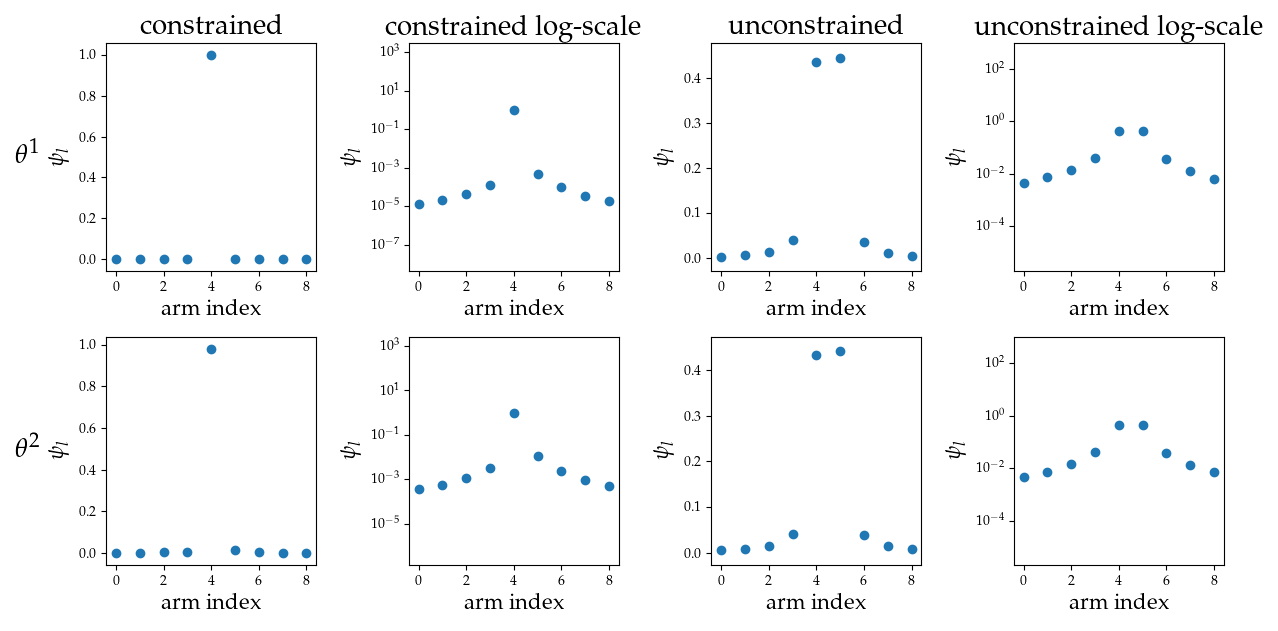
\includegraphics[width=\textwidth]{optimal_allocation.png}
  \caption{Unconstrained and constrained optimal allocation for $\theta_1$ and $\theta_2$, top-4}
  \label{fig:optimal_allocation}
\end{figure}

TODO: Propose an intuition why the concentration is so high in unconstrained scenario.

\section{Proofs}\label{section:optimal_proofs}
\begin{proof}[\Cref{lemma:set_relation_S*_i}]
  We first show the relationship between $\Theta_{S^*}^c$ and sets $\bar{\Theta}_i$ and then show the relationship between $\Theta_{S^*}^c$ and $\Theta_j$.
  \begin{align}
    \Theta_{m, S^*}^c &= \{\theta \in \Theta | \min_{j \in S^*} \theta_j > \max_{i \notin S^*} \theta_i \}^c \\
    &= \{\theta \in \Theta | \max_{i \notin S^*} \theta_i \geq \min_{j \in S^*} \theta_j\} \\
    &= \{\theta \in \Theta | \exists i \notin S^*: \theta_i \geq \min_{j \in S^*} \theta_j\} \\
    &= \{\theta \in \Theta | \exists i \notin S^*: \text{top-}m(\theta, S^* \cup \{i\}) \neq S^*\} \\
    &= \bigcup_{i \notin S^*} \{\theta \in \Theta | \text{top-}m(\theta, S^* \cup \{i\}) \neq S^*\} \\
    &= \bigcup_{i \notin S^*} \bar{\Theta}_i \\
    \Theta_{m, S^*} &= \{\theta \in \Theta | \min_{j \in S^*} \theta_j > \max_{j \in S^*} \theta_j\} \\
    &= \{\theta \in \Theta | \bigwedge_{j \in S^*} \theta_j > \max_{j \in S^*} \theta_j\} \\
    &= \bigcap_{j \in S^*} \{\theta \in \Theta | \theta_j > \max_{j \in S^*} \theta_j\} \\
    &= \bigcap_{j \in S^*} \{\theta \in \Theta | j \in \text{top-}m(\theta, [k])\} \\
    &= \bigcap_{j \in S^*} \Theta_j \\
    \Theta_{m, S^*}^c &= \Theta - \Theta_{m, S^*}\\
    \Theta_{m, S^*}^c &= \Theta - \bigcap_{j \in S^*} \Theta_j
  \end{align}
\end{proof}

\begin{proof}[\Cref{lemma:posterior_S*_i}]
  First, we prove the equality for $i \notin S^*$, followed by the equality for $j \in S^*$.

  The union from \Cref{lemma:set_relation_S*_i} has an additive effect with respect to the probability distribution $\Pi_n$. There are $k-m$ possible $i$s and each single one leads to a set, whose density is bounded by the maximal density of all such sets. This gives us:
  \begin{align}
    \max_{i \notin S^*} \Pi_n(\bar{\Theta}_i) \leq \Pi_n(\Theta_{m, S^*}^c) \leq (k-m) \max_{i \notin S^*} \Pi_n(\bar{\Theta}_i)
  \end{align}
  We use the definition of $\deq$ to check whether lower bound and upper bound are equal.
  \begin{align}
    \lim_{n \rightarrow \infty} \frac{1}{n} \log{\frac{\max_{i \notin S^*} \Pi_n(\bar{\Theta}_i)}{(k-m)\max_{i \notin S^*} \Pi_n(\bar{\Theta}_i)}}
    = \lim_{n \rightarrow \infty} \frac{1}{n} \log{\frac{1}{k-m}} \rightarrow 0
  \end{align}
  Thanks to the lower and upper bound being equal in the $\deq$ sense, we can apply the squeeze theorem. We obtain the desired result:
  \begin{align}
    \Pi_n(\Theta_{m, S^*}^c) \deq \max_{i \notin S^*} \Pi_n(\bar{\Theta}_i)
  \end{align}
  For $j \in S^*$, we follow a very similary path by first leveraging the set equality from \Cref{lemma:set_relation_S*_i}. Instead of a union, as was the case for $i \in S^*$, we are now confronted with an intersection. This implies a mulitplicative effect on the distribution $\Pi_n$ instead of an additive one.
  \begin{align}
    &1 - \min_{j \in S^*} \Pi(\Theta_j) \leq \Pi(\Theta_{m, S^*}^c) \leq 1 - \min_{j \in S^*} (\Pi(\Theta_j))^m \\
  \end{align}
  Again, we will check whether upper and lower bound equal in the $\deq$ sense.
  \begin{align}
    &\lim_{n \rightarrow \infty} \frac{1}{n} \log(\frac{\min_{j \in S^*} \Pi(\Theta_j)}{\min_{j \in S^*} (\Pi(\Theta_j))^m}) = \lim_{n \rightarrow \infty} \frac{-(m - 1)}{n} \log(\min_{j \in S^*} \Pi(\Theta_j))
  \end{align}
  Observe that $1 \geq \min_{j \in S^*} \Pi(\Theta_j) \geq \alpha_{n, S^*} \rightarrow 1$. Hence the limit of the fraction goes to 0 and we have $\min_{j \in S^*} \Pi(\Theta_j) \deq \min_{j \in S^*} (\Pi(\Theta_j))^m$. Applying, by the Squeeze theorem it follows that
  \begin{align}
    \Pi_n(\Theta_{m, S^*}^c) \deq 1 - \min_{j \in S^*} \Pi_n(\Theta_j)
  \end{align}
\end{proof}

\begin{proof}[\Cref{lemma:kl_to_C}]
  \begin{align}
    \min_{\theta \in \bar{\Theta}_i} D_\psi(\theta^*||\theta) &= \min_{\theta \in \bar{\Theta}_i} \sum_{j=1}^k \psi_j d(\theta^*_j||\theta_j)\\
    &= \min_{\theta \in \bar{\Theta}_i} \sum_{j\in S^*} \psi_{j}d(\theta^*_{j} || \theta_{j}) + \psi_{i}d(\theta_{i}^* || \theta_{i}) + \sum_{j \notin S^* \cup \{i\}} \psi_j d(\theta^*_j||\theta_j) \\
    &= \min_{\theta \in \bar{\Theta}_i} \sum_{j\in S^*} \psi_{j}d(\theta^*_{j} || \theta_{j}) + \psi_{i}d(\theta_{i}^* || \theta_{i}) \label{eq: l2_1}\\
    &= \min_{j\in S^*} \min_{\theta \in \bar{\Theta}_i} \psi_{j}d(\theta^*_{j} || \theta_{j}) + \psi_{i}d(\theta_{i}^* || \theta_{i}) \label{eq: l2_2}\\
    &= \min_{j\in S^*} \min_{\theta \in \bar{\Theta}_i} \psi_{j}d(\theta^*_{j} || \theta_{j}) + \psi_{i}d(\theta_{i}^* || \theta_{j}) \label{eq: l2_3}\\
    &= \min_{j\in S^*} \min_{x \in \mathbb{R}} \psi_{j}d(\theta^*_{j} || x) + \psi_{i}d(\theta_{i}^* ||x) \label{eq: l2_4}\\
    &= \min_{j \in S^*} C_{j, i}(\psi_j, \psi_i)
  \end{align}
  \eqref{eq: l2_1} follows from the fact that for any feasible $\theta$, we can define an alternative $\theta'$ s.t. $\theta'_i = \theta_i$, $\theta'_j = \theta_j$ for all $j \in S^*$ and $\theta'_{i_x} = \theta^*_{i_x}$ for all $i_x \notin S^* \cup \{i\}$. For such a $\theta'$, all terms involving $i_x \notin S^* \cup \{i\}$ are zero by the definition of the KL divergence while all others terms remain unchanged. Hence the minimum occurs with such a $\theta'$. Importantly, $\theta'$ remains feasible according to current definitions of $\bar{\Theta}_i$, i.e. $\theta' \in \bar{\Theta}_i$.

  \eqref{eq: l2_2} follows from a similar observation: only a single arm from $S^*$ needs to be inferior to arm $i$ under $\theta$. Recall that the terms of the individual arms do not influence each other. This implies that the minimization will gravitate towards setting all but one arm from $S^*$ in $\theta$ to the their true value - as the KL divergence is minimized for those values. Hence the terms of all but one arm from $S^*$ will be cancelled out by the minimization. As $i$ remains superior to one arm in $S^*$, we have top-$m(\theta, S^* \cup \{i\}) \neq S^*$. Thereby such a $\theta$ is feasible according to $\bar{\Theta}_i$.

  \eqref{eq: l2_3} follows from monotonicity of the KL divergence, as displayed in \Cref{eq:kl_monotonicity}, combined with the possibility of $\theta_i = \theta_j$ tells us that the minimum will be reached in the case of equality.

  \eqref{eq: l2_4} follows from observing that our minimization over $\theta$ has reduced to a minimization over $\theta_j$. The latter is a one-dimensional real.
\end{proof}

\begin{proof}[\Cref{lemma:C_concave}]
  For the sake of clarity, let us define $f(x, (\psi_j, \psi_i)) = \psi_j d(\theta_i^*||x) + \psi_i d(\theta_i^* || x)$. Note that $C_{j, i}(\psi_j, \psi_i) = min_{x \in \mathbb{R}} f(x,(\psi_j, \psi_i))$. Clearly, $f$ is linear in $(\psi_j, \psi_i)$. According to Boyd and Vandenberghe (3.2.5) \cite{Boyd:2004:CO:993483}, the minimum over a family of linear functions is concave.
\end{proof}

\begin{proof}[\Cref{lemma:C_unique_solution}]
  By \Cref{eq:exponential_kl} we know that for the exponential family of probability distributions it holds that:
  \[d(\theta||\theta') = (\theta - \theta')A'(\theta) - A(\theta) + A(\theta')\]
  Appyling this identity to \eqref{eq: l2_4} for a given $j$ gives us:
  \begin{align}
    &\psi_{j}d(\theta^*_{j} || x) + \psi_{i}d(\theta_{i}^* ||x) \\
    &=\psi_j ((\theta_j^* - x)A'(\theta_j^*) - A(\theta_j^*) + A(x)) + \psi_i((\theta_i^* - x)A'(\theta_i^*) - A(\theta_i^*) + A(x))\\
    &= -x(\psi_j A'(\theta_j^*) + \psi_i A'(\theta_i^*)) + A(x)(\psi_j + \psi_i) + c
  \end{align}
  Where $c$ is independent of $x$. As we seeks to minimize this quantity with respect to $x$, we differentiate it with respect to $x$ and set it to 0. This yields:
  \[A'(x) = \frac{\psi_j A'(\theta_j^*) + \psi_i A'(\theta_i^*)}{\psi_j + \psi_i}\]
\end{proof}

\begin{proof}[\Cref{proposition:characterization}]
  We prove in the following order: \eqref{itm:p7_i} \eqref{eq:condition_C} must hold for an optimal allocation, \eqref{itm:p7_ii} an optimal allocation is unique, \eqref{itm:p7_iii} what the convergence rate of the optimal allocation is and \eqref{itm:p7_iv} that none can do better.
  \begin{enumerate}[(i)]
    \item \label{itm:p7_i} Suppose that $\psi^*$ is optimal but does not satisfy \eqref{eq:condition_C}. Hence for some $i_1, i_2 \notin S^*, j_1, j_2 \in S^*$ with $(j_1, i_1) \neq (j_2, i_2)$:
    \[C_{j_1, i_1}(\psi^*_{j_1}, \psi^*_{i_1}) > C_{j_2, i_2}(\psi^*_{j_2}, \psi^*_{i_2})\]
    This implies:
    \[C_{j_1, i_1}(\psi^*_{j_1}, \psi^*_{i_1}) > \min_{i \notin S^*} \min_{j \in S^*}C_{j, i}(\psi^*_j, \psi^*_i) \]
    Consider the the measurement plan $\psi^\epsilon$ with
    \begin{itemize}
      \item $\psi^\epsilon_{i_1} = \psi^*_{i_1} - \epsilon$
      \item $\psi^\epsilon_{j_1} = \psi^*_{j_1} - \epsilon$
      \item $\forall l\notin \{i_1, j_1\}: \psi^\epsilon_l = \psi^*_\gamma + \frac{2 \epsilon}{k-2}$
    \end{itemize}
    We can choose $\epsilon$ sufficiently small such that we preserve the inequality
    \begin{align}
      C_{j_1, i_1}(\psi^\epsilon_{j_1}, \psi^\epsilon_{i_1}) > C_{j_2, i_2}(\psi^\epsilon_{j_2}, \psi^\epsilon_{i_2})
    \end{align}
    while shifting enough measurement to all other arms such that
    \begin{align}
      \min_{i \notin S^*} \min_{j \in S^*} C_{j, i}(\psi^\epsilon_{j}, \psi^\epsilon_i) > \min_{i \notin S^*} \min_{j \in S^*} C_{j, i}(\psi^*_j, \psi^*_i)
    \end{align}
    Hence $\psi^\epsilon$ obtains more evidence on the worst possible pair than $\psi^*$ and thereby achieves a better convergence rate \eqref{eq:constrained_optimal_gamma}. In other words, $\psi^*$ is not optimal, which is a contradiction.

    \item \label{itm:p7_ii} Suppose that there are optimal $\psi^1$, $\psi^2$, therefore both satisfying \eqref{eq:condition_C} with the exact same value $C^*$. It follows that there is at least one $l$ s.t. $\psi^1_{l} \neq \psi^2_{l}$. W.l.o.g. assume $l = i_x \notin S^*$ and $\psi^1_{i_x} > \psi^2_{i_x}$.

    We proceed by case distinction and show that each leads to a contradiction.
    \begin{itemize}
      \item Only one arm is disinct.

      For some $\epsilon > 0$ and any $j \in S^*$ have
      \begin{align}
        C_{j, i_x}(\psi^2_j, \psi^2_{i_x} + \epsilon) &= C_{j, i_x}(\psi^1_j, \psi^2_{i_x} + \epsilon) \\
        &= C_{j, i_x}(\psi^1_j, \psi^1_{i_x}) \\
        &= C^* \\
        &= C_{j, i_x}(\psi^2_j, \psi^2_{i_x})
      \end{align}
      Which is a contradiction as $\epsilon$ is positive $C_{j, i_x}$ monotonically increasing.
      \item More that one arm is distinct, but they all belong to either $S^*$ or $S^{*c}$.

      As our distinct value so far comes from $S^{*c}$, let's also assume, w.l.o.g., $i_y \notin S^*$ with $i_y \neq i_x$.

      Note that indepdently of whether $\psi^1_{i_y} \geq \psi^2_{i_y}$ or $\psi^1_{i_y} < \psi^2_{i_y}$ holds, the previous argument can be applied for any $j \in S^*$.

      \item At least one arm is distinct in both $S^*$ and $S^{*c}$.

      Let's assume first that the distinctive optimal arm is $j_x \in S^*$. Observe that $\psi^1_{j_x} < \psi^2_{j_x}$ has to hold, otherwise both $i_x$ and $j_x$ were allocated more weight in $\psi^1$ than in $\psi^2$. By the monotonicity of $C_{j_x, i_x}$, this would imply greater evidence for $\psi^1$ than for $\psi^2$, a contradiction to the assumption that both are optimal.

      Recall our constraint $\frac{1}{2} = \sum_{j \in S^*} \psi_l = \sum_{i \notin S^*} \psi_i$, which has to hold for both $\psi^1$ and $\psi^2$.
      Hence for $psi^1$'s over-allocation on $i_x$, there has to be an $i_y \notin S^*$ for which $\psi^1$ under-allocates, compared to $psi^2$.
      Summarizing, we have:
      \begin{itemize}
        \item $\psi^1_{i_x} = \psi^2_{i_x} + \epsilon$
        \item $\psi^1_{j_x} = \psi^2_{j_x} - \epsilon'$
        \item $\psi^1_{i_y} = \psi^2_{i_y} - \epsilon''$
      \end{itemize}
      Combining this with the fact that all $C$ values from both $\psi^1$ and $\psi^2$ have to equal one another, we obtain:
      \begin{align}
        C_{j_x, i_y}(\psi^2_{j_x} - \epsilon', \psi^2_{i_y} - \epsilon'') &= C_{j_x, i_y}(\psi^1_{j_x}, \psi^1_{i_y}) \\
        &= C^* \\
        C_{j_x, i_y}(\psi^2_{j_x}, \psi^2_{i_y})
      \end{align}
      which, again, is a contradiction by the monotonicity of the KL divergence.
    \end{itemize}

    $l$ is either inside or outside of $S^*$. As both cases are analogous, let's assume $l = j_x \in S^*$. Combining the knowledge of \eqref{eq:condition_C} and $C_{j, i}$ being stictly increasing in the first argument leads to $C_{j_x, i}(\psi^1_{j_x}, \psi^1_i) > C_{j_x, i}(\psi^2_{j_x}, \psi^2_i)$ for all $i \notin S^*$. Hence $\psi^2$ is not optimal, which is a contradiction.

  \item \label{itm:p7_iii}
  \item \label{itm:p7_iv}
  \end{enumerate}

\end{proof}

\chapter{Algorithm}
\section{Analysis/Properties}
\section{Empirical behaviour}\label{section:empirical_behaviour}
What true distributions are assumed?
What prior and posterior distributions are assumed?
How is C computed?
How is alpha computed, as it is defined via a huge integral?
How is psi computed, as there is no closed form?
\section{Proofs}

\chapter{Conclusion}


\appendix

\chapter{Appendix}

\section{Computing $C_{j, i}$ for Bernoulli means}\label{section:bernoulli_c}

We assume that every arm $l$ follows a Bernoulli distribution with parameter $\theta_l$. The option space for rewards being $\{0, 1\}$, they are discretely distributed. Let us reiterate the definition of the KL divergence for discrtete distributions:
\[d(p || q) = \sum_{y \in Y}p(y) \log(\frac{p(y)}{q(y)})\]
where $Y$ corresponds the option space for the outcome.
Instantiating this definition with our scenario, we observe that $Y=\{0, 1\}$, $p(y=1)=\theta_l$  as well as $p(y=0)=1-\theta_l$, for a given arm $l$.

This yields:
\begin{align}
  d(\theta_l||x) = \theta_l \log(\frac{\theta_l}{x}) + (1-\theta_l) \log(\frac{1-\theta_l}{1-x}) \label{eq:bernoulli_kl}
\end{align}
Recall that for computing $C_{j, i}$, we seek to minimize the expression from \eqref{eq:C} $x \in \mathbb{R}$. Hence we are interested in the derivative of \eqref{eq:bernoulli_kl} with respect to $x$.
\begin{align}
  \diff{(d(\theta_l||x)}{x} &= - \frac{\theta_l}{x} + \frac{(1-\theta_l)}{1-x}
\end{align}
Drawing from the minimization problem of $C_{j,i}$ for given $j$, $i$, $\psi_j$ and $\psi_i$, we define $f(x) = \psi_j d(\theta^*_{j} || x) + \psi_i d(\theta_{i}^* ||x)$. We proceed by deriving $f$ with respect to $x$ and setting it to 0.
\begin{align}
  \diff{f(x)}{x} &= \psi_j(\frac{\theta_j}{x} + \frac{(1-\theta_j)}{1-x}) + \psi_i( \frac{\theta_i}{x} + \frac{(1-\theta_i)}{1-x}) \\
  &= -\frac{1}{x}(\psi_j\theta_j + \psi_i\theta_i) + \frac{1}{1-x}(\psi_j(1 - \theta_j) + \psi_i(1 - \theta_i)) \\
  \diff{f(x)}{x} = 0 &\Rightarrow (1-x_0)(\psi_j\theta_j + \psi_i\theta_i) = x_0(\psi_j(1 - \theta_j) + \psi_i(1 - \theta_i))\\
  &\Rightarrow x_0((\psi_j\theta_j + \psi_i\theta_i) + (\psi_j(1 - \theta_j) + \psi_i(1 - \theta_i))) = (\psi_j\theta_j + \psi_i\theta_i)\\
  &\Rightarrow x_0 = \frac{\psi_j\theta_j + \psi_i\theta_i}{(\psi_j\theta_j + \psi_i\theta_i) + (\psi_j(1 - \theta_j) + \psi_i(1 - \theta_i))} \\
  &\Rightarrow x_0 = \frac{\psi_j\theta_j + \psi_i\theta_i}{\psi_j + \psi_i}
\end{align}
Hence we have a very intuitive analytical solution for $x$: it is an average of the means of $j$ and $j$, weighted by their respective measurement allocation.

\section{Facts about the exponential family}
%TODO:Explain what A, A' and theta represent.
%TODO:Doublecheck correctness of A' via wikipedia
Russo presents the following insight about the exponential family of probability distributions.
\begin{itemize}
  \item Its log-partition-function $A(\theta)$ is strictly convex and differentiable.
  \item Its mean equals $A'(\theta) = \int T(y)p(y|\theta)d\nu(y)$.
  \item The KL divergence equals:
    \begin{align}
        d(\theta||\theta') = (\theta - \theta')A'(\theta) - A(\theta) + A(\theta')\label{eq:exponential_kl}
    \end{align}
  \item The KL divergence satisfies:
    \begin{align}
      &\theta'' > \theta' \geq \theta \Rightarrow d(\theta||\theta'') > d(\theta||\theta') \label{eq:kl_monotonicity}\\
      &\theta'' < \theta' \leq \theta \Rightarrow d(\theta||\theta'') < d(\theta||\theta')
    \end{align}
\end{itemize}


\backmatter

\bibliographystyle{plain}
\bibliography{refs}

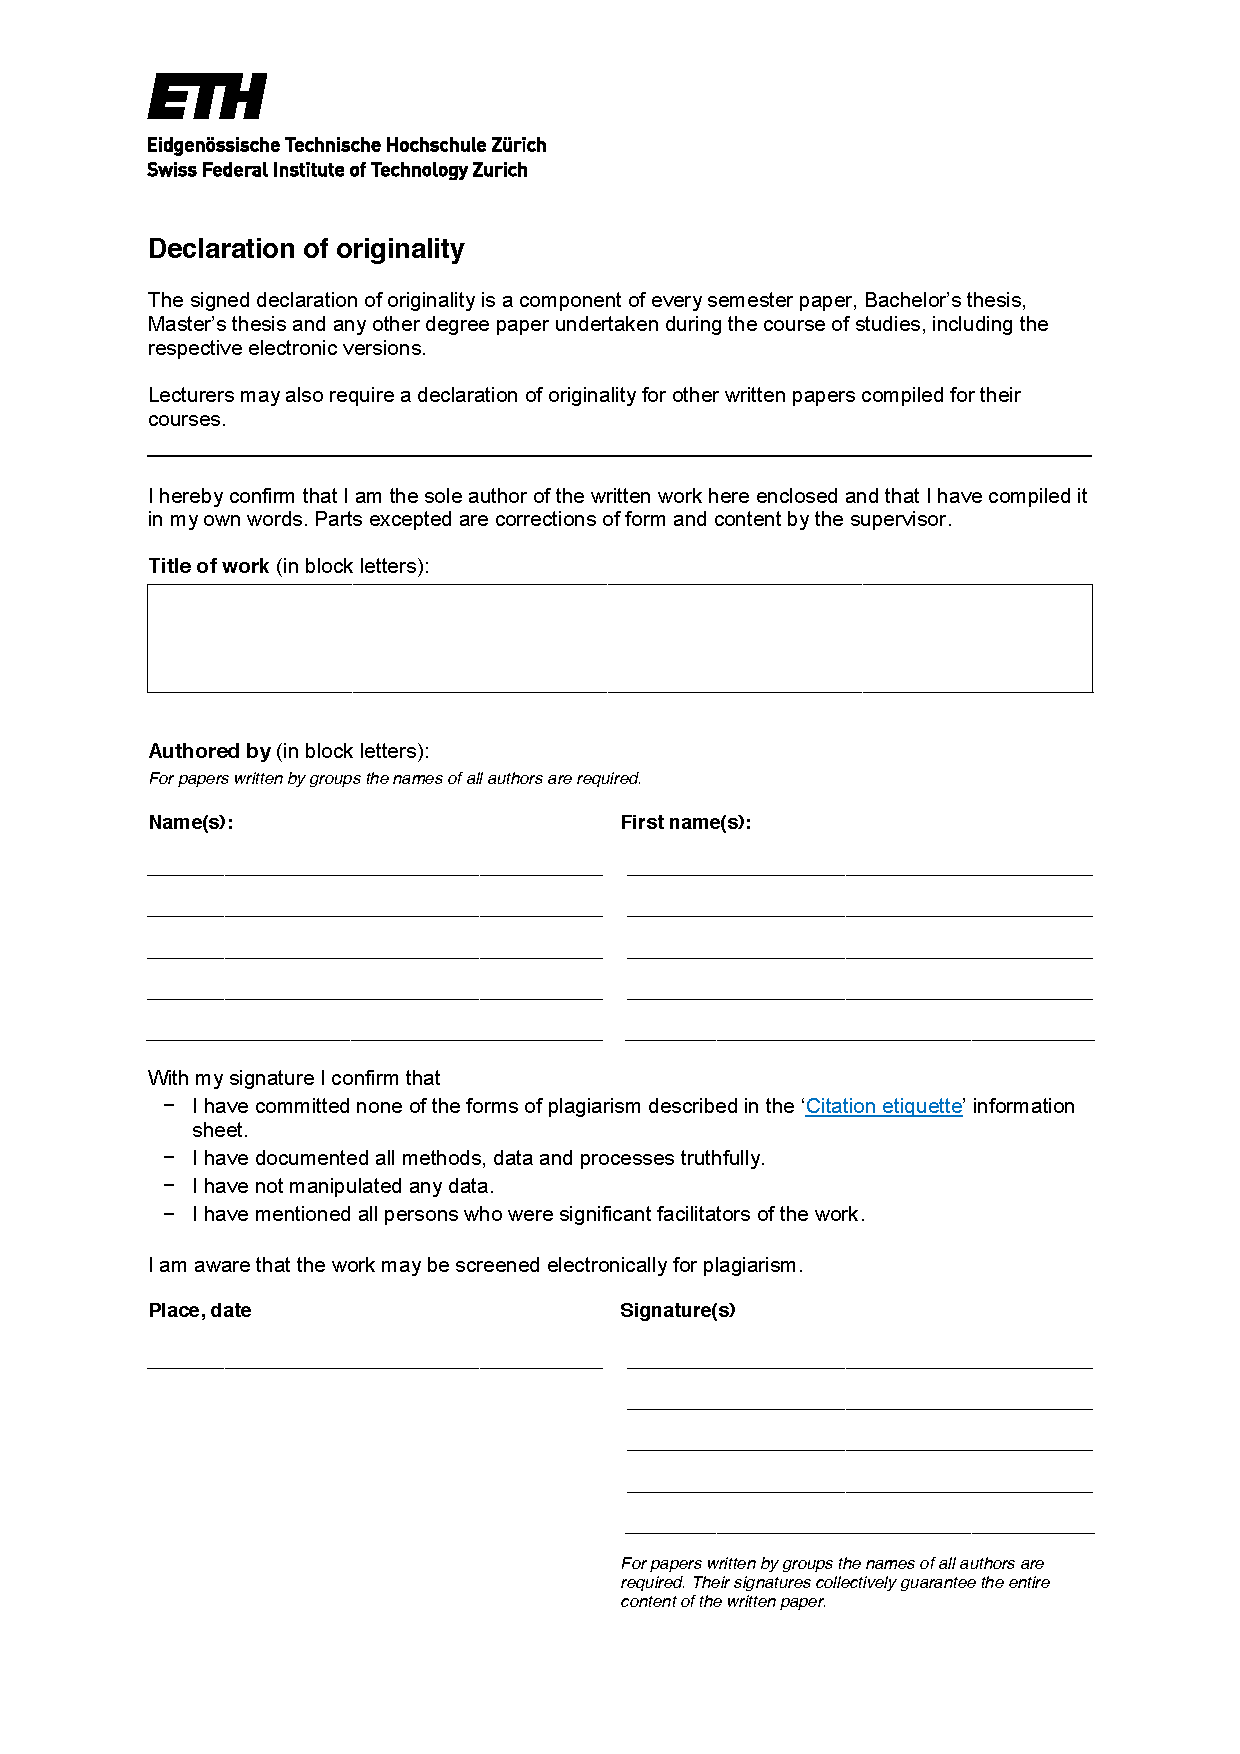
\includepdf[pages={-}]{declaration-originality.pdf}

\end{document}
